% Created 2019-06-27 木 15:54
% Intended LaTeX compiler: pdflatex
\documentclass{article}

\usepackage{authblk}

% \usepackage[dvipdfmx]{graphicx}
\usepackage{graphicx} % We removed [dvipdfmx] option because the figure in PDF format did not display.

\date{}
\title{Every Reconfiguration Starts with a First Step}
\pagenumbering{gobble}

\author[1]{Akira Suzuki}
\affil[1]{Graduate School of Information Sciences, Tohoku University}

\begin{document}
\maketitle

\section{Our instance for (graph\#10) track}
	\begin{figure}[t]
		\begin{tabular}{cc}
			\begin{minipage}[t]{0.5\hsize}
				\centering
				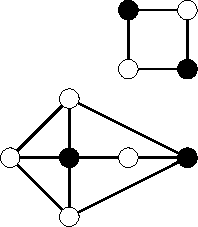
\includegraphics{10_s.pdf}
			\end{minipage}
		&
			\begin{minipage}[t]{0.5\hsize}
				\centering
				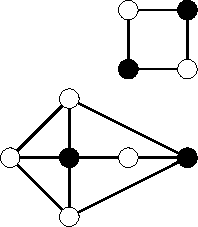
\includegraphics{10_t.pdf}
			\end{minipage}
		\\
		(a)
		&
		(b)
		\end{tabular}
		\caption{Our instance for (graph\#10) track, (a) the initial independent set, and (b) the target independent set.}
		\label{figure_10instance}
	\end{figure}
	\begin{figure}[t]
		\begin{tabular}{c}
			\begin{minipage}[t]{1.0\hsize}
				\centering
				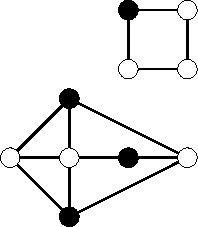
\includegraphics{10_m.pdf}
			\end{minipage}
		\end{tabular}
		\caption{The independent set of four steps after the initial solution. Since there are three tokens on the kite, we can move the token on the $C_4$.}
		\label{figure_10mid}
	\end{figure}
	\begin{itemize}
	\item A completely handcrafted instance, as shown in Figure~\ref{figure_10instance}. Our graph has two parts: the $C_4$ part above and the ``kite'' part below.
	\item The only difference between the initial and the target solutions is the two tokens on the $C_4$. However, these tokens interfere with each other, so they cannot be changed directly on the $C_4$ alone. Therefore, first, we need to move one of these tokens onto the kite, using four steps. (See Figure~\ref{figure_10mid}.)
	\item After reconfiguring the tokens on the $C_4$, we need to replay the previous step in reverse to restore the tokens on the kite, so the reconfiguration takes a total of nine steps.
	\end{itemize}

\section{Our instance for (graph\#50) track}
	\begin{figure}[t]
		\begin{tabular}{cc}
			\begin{minipage}[t]{0.5\hsize}
				\centering
				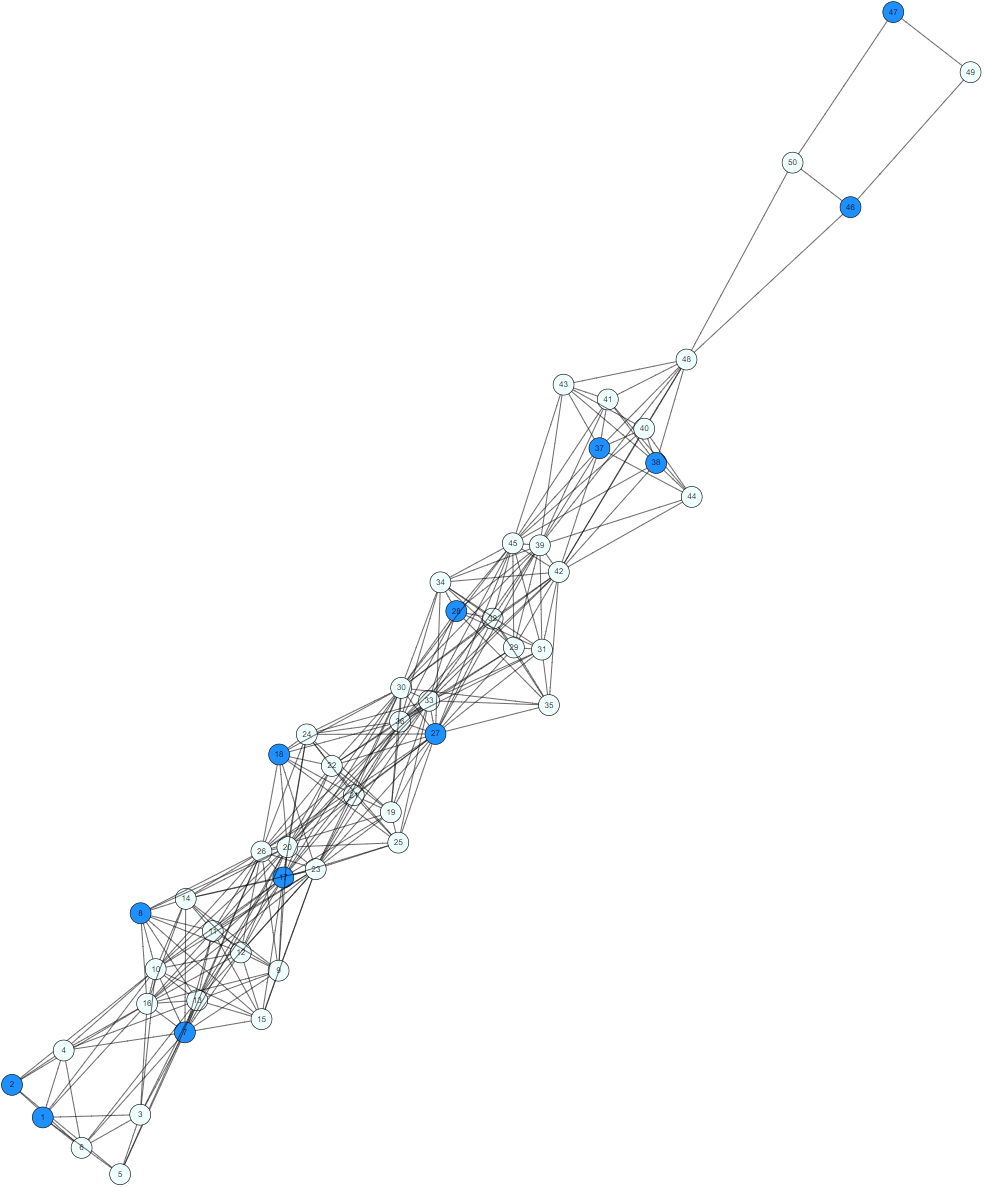
\includegraphics[scale=0.2]{50_s.png}
			\end{minipage}
		&
			\begin{minipage}[t]{0.5\hsize}
				\centering
				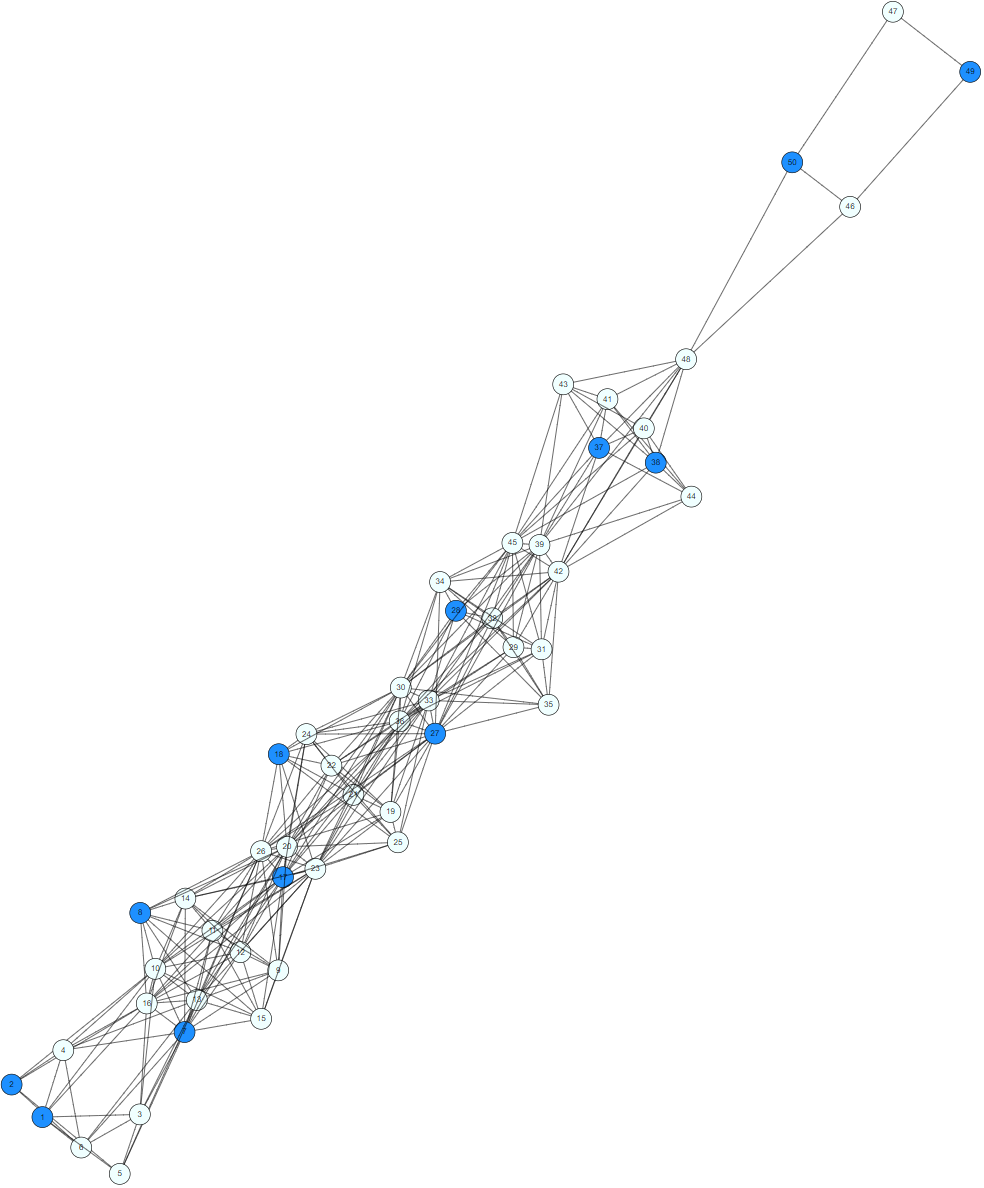
\includegraphics[scale=0.2]{50_t.png}
			\end{minipage}
		\\
		(a)
		&
		(b)
		\end{tabular}
		\caption{Our instance for (graph\#50) track, (a) the initial independent set, and (b) the target independent set.}
		\label{figure_50instance}
	\end{figure}
\begin{itemize}
\item Our instance is shown in Figure~\ref{figure_50instance}. It contains 50 vertices and 263 edges.
\item We use the same idea as in our previous paper: Akira Suzuki, Amer E. Mouawad and Naomi Nishimura, Reconfiguration of dominating sets, Journal of Combinatorial Optimization 32(4), pp. 1182--1195, 2016.
\item The only difference between the initial and the target solutions is the top right two tokens of Figure~\ref{figure_50instance}.
\item However, 643 steps are required before and after reconfiguring these two tokens. Then the total reconfiguration takes 1,289 steps.
\end{itemize}

\section{Our instance for (graph\#100) track}
	\begin{figure}[t]
		\begin{tabular}{c}
			\begin{minipage}[t]{1.0\hsize}
				\centering
				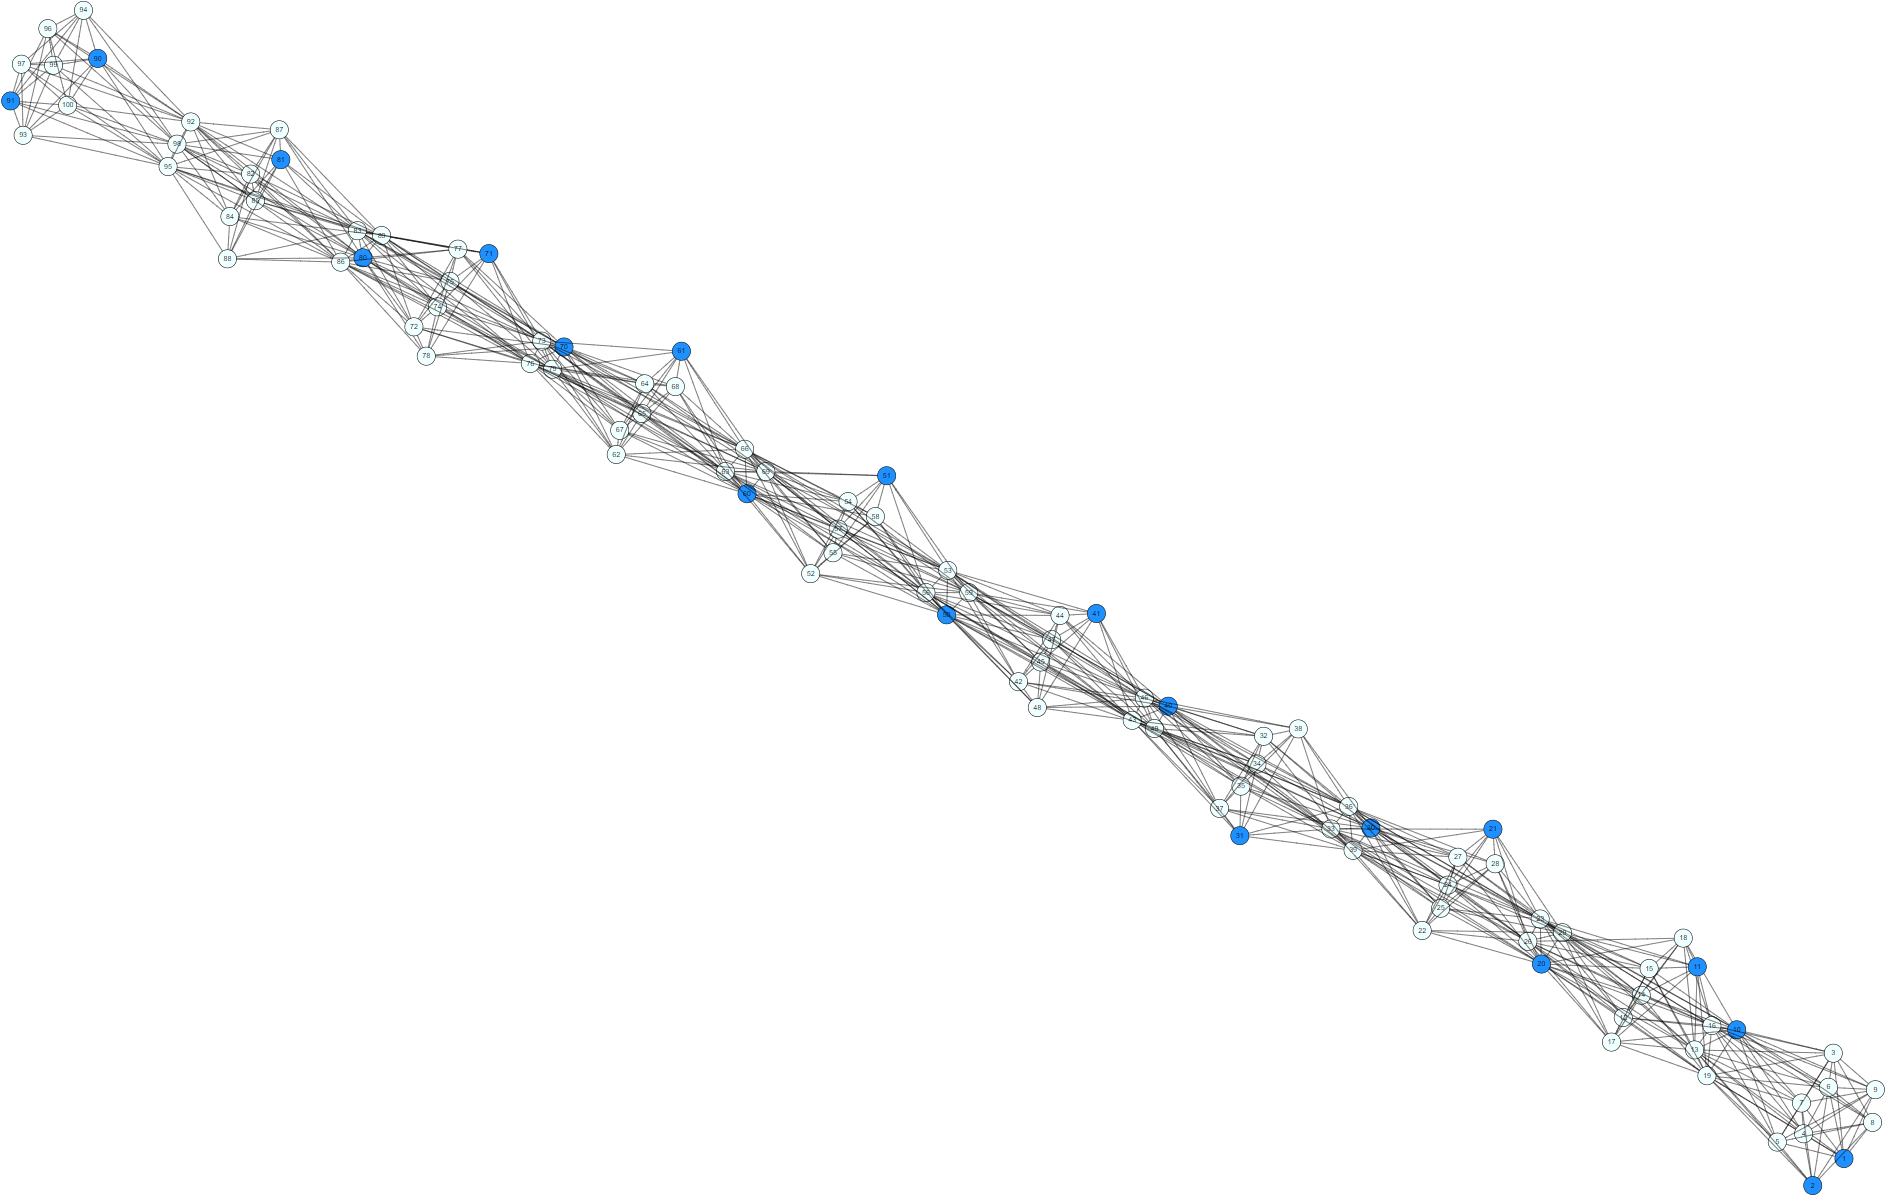
\includegraphics[scale=0.2]{100_s.png}
			\end{minipage}
		\\
		(a)
		\\
			\begin{minipage}[t]{1.0\hsize}
				\centering
				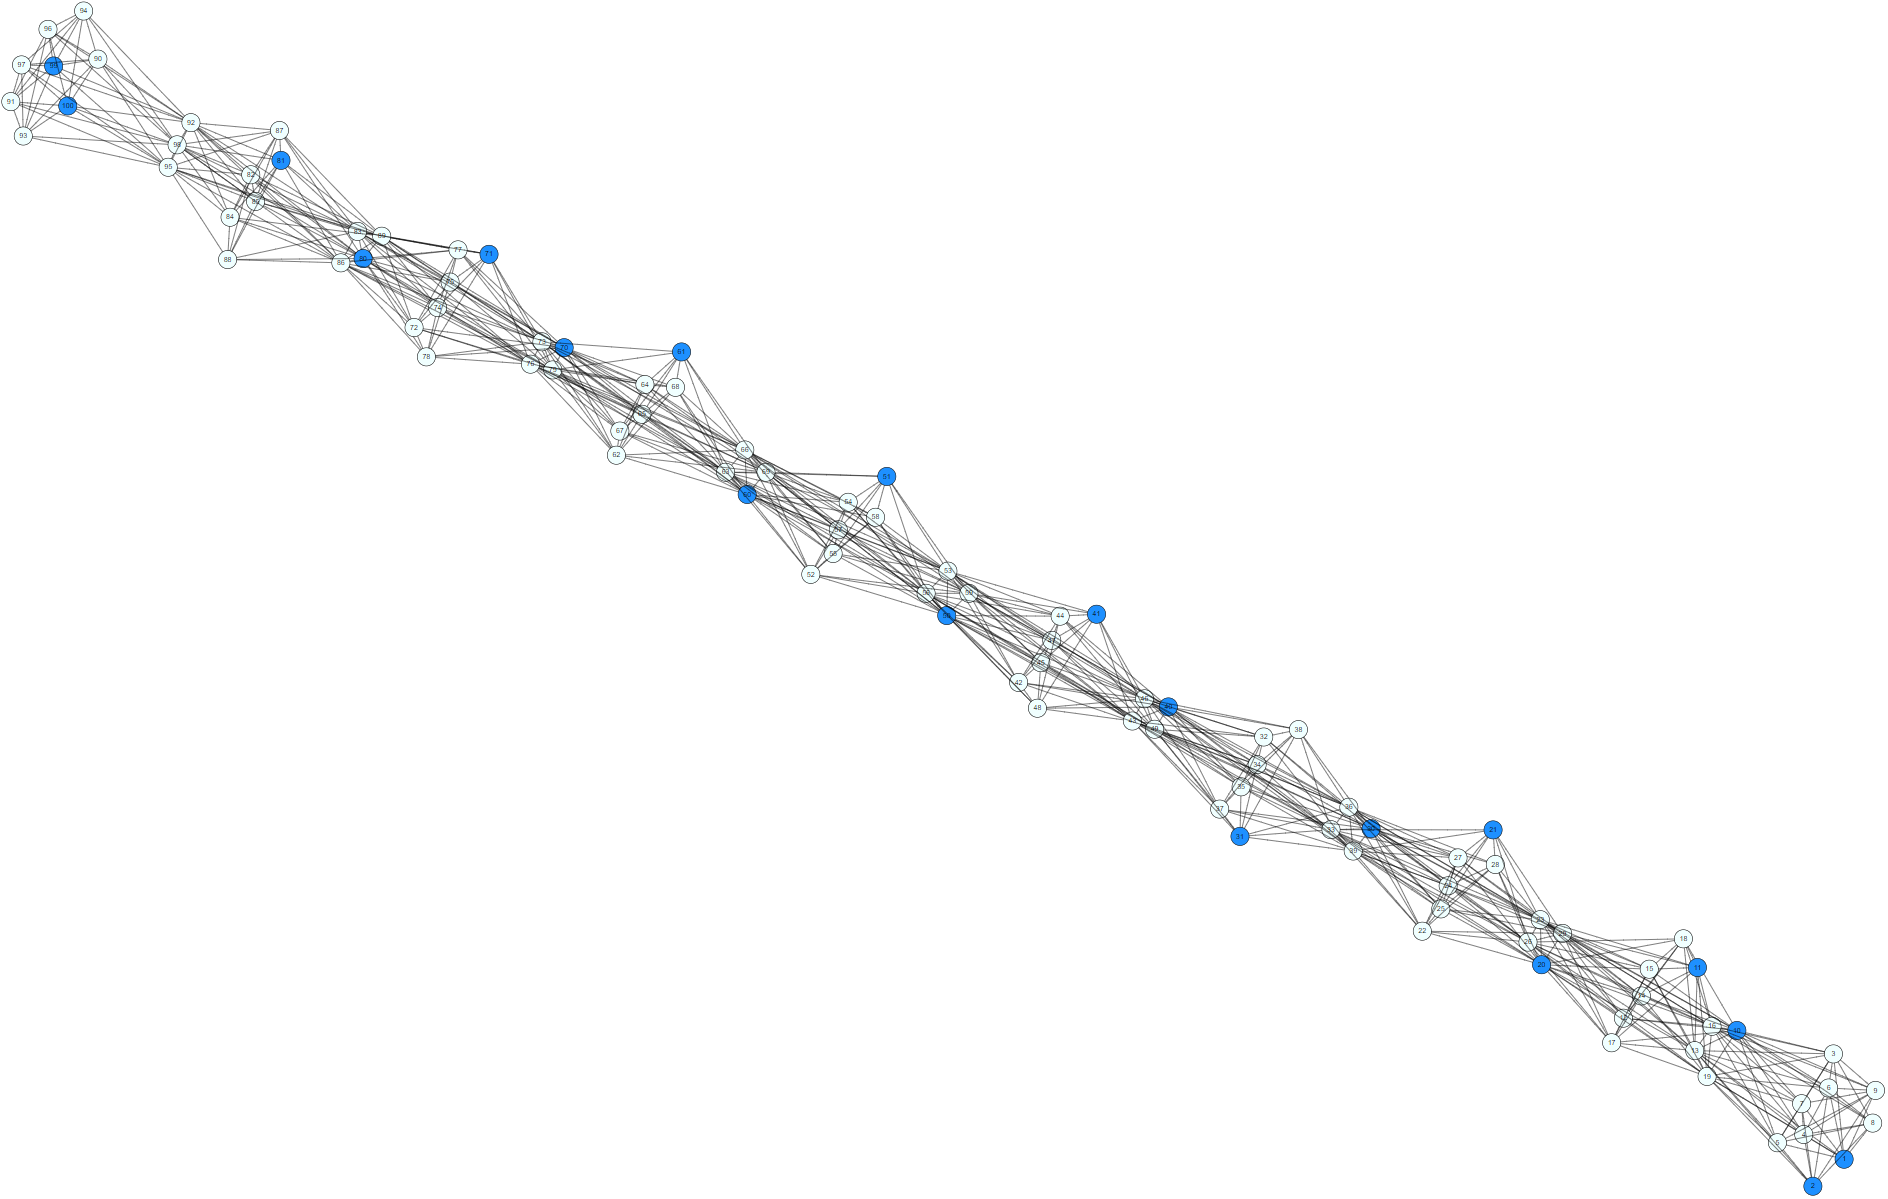
\includegraphics[scale=0.2]{100_t.png}
			\end{minipage}
		\\
		(b)
		\end{tabular}
		\caption{Our instance for (graph\#100) track, (a) the initial independent set, and (b) the target independent set.}
		\label{figure_100instance}
	\end{figure}
\begin{itemize}
\item Our instance is shown in Figure~\ref{figure_100instance}. It contains 100 vertices and 637 edges.
\item The idea is the same as (graph\#50): While the only difference between the initial and the target solutions is the top left two tokens of Figure~\ref{figure_100instance}, the total reconfiguration takes 288,677 steps.
\end{itemize}

\end{document}